%Settings{{{
\documentclass[12pt]{iopart}
\usepackage{graphicx}
\usepackage{iopams}

% Fixing iopams poor centering of equations:
\expandafter\let\csname equation*\endcsname\relax
\expandafter\let\csname endequation*\endcsname\relax
\usepackage{amsmath}
\usepackage{gensymb}
%
%}}}

%Plan {{{ 
% Title
%% Make sure that I only talk about areas I am really interested in and want to talk about. 


%% State of the art experimental apparatus for fast entangling gates in trapped multi-ion crystals

%% 11 Page limit

%% (Short) intro to trapped ion QC and Theory on Fast Gates schemes: ~ 2 pages

%%     * Motivating why QC important. ~ 1 paragraph

%%     * Trapped Ion QC - General idea of spin (ion) coupled with HO (Trapping potential) and how this satisfies QC requirements. ~ 1-2 paragraph

%%     * Entangling gates MS gate. Statement of Hamiltonian and how this is experimentally realised. ~ 1 paragraph

%%     * Fast Gate Schemes (Non-Adiabatic Entanglement). Amplitude shaped pulses. ~ 1 sentence and reference
%%         Why we want to move to quadrupole optical transition rather than Raman (Scattering error and squeezing term)

%%     * Carrier Nulling. (excerpt from paper starts) ~ 2 paragraphs

 

%% Experimental results from Carrier Nulling (excerpts from paper): ~ 2+ pages

%%     * Description of Blade ~ 1 figure + 1 paragraph

%%     * Phase control ~ 1 paragraph

%%     * Proof of principle on Blade apparatus ~ 2 paragraph (statement of results) 2 figures

%%     RBM work ~ few sentences

 

%% FastGates buildup: ~ 4 pages

%%     * Motivation for why we want a new system (compare with Blade) ~ 1 paragraph

%%     * Description of FastGates – central figure of full physical experiment and figure of control systems ~ 2 paragraphs large figure
%%         In effect list all the benefits over Blade - and how it fits into requirements for NISQ?

%%     Now looking at components of new system from center outward:

%%     * Ca40 energy diagram  ~ 1 paragraph and energy level figure
%%         Simple energy structure. Less spectator modes compared to Ca43 -> less off resonant transitions. But sensitive to B field.

%%     * NPL trap, trap frequencies, substrate bias for crystal rotation ~ 1 paragraph 1 figure
%%         What trap freq do we want for fast gates 

%%     * In vacuum system details ~ 1 paragraph 1 figure

%%     * Dual Optical Access High NA system ~ few sentences

%%     * Single Ion Addressing with AOD, power requirements ~ 1 paragraph
%%         This is potentially a drain of time – time bound looking into this.

%%     * Addressing and Readout optics design? ~ short 1 figure

%%     * Extension to standing wave single ion addressing – ideas/design for phase feedback ~ few sentences 1 figure?

%%     * 729 system design, PDH locking, FNC ~ 1 paragraph

   

%% Outlook: ~ 1 page

%%     * Overall goals of project
%%         - Optical phase control of laser field at the ion.
%%         - Fastgates on multi ion chain.

%%     * Immediate tasks: Finishing vacuum work, trap on table. Trapping ions 

%%     * Proposed first experiments? 
%%         1st paper: EOM to keep stark shift the same as pulse amplitude changes 
%%         Explore this for 1 day
%%             Ask about scheme 
%%             This is a problem with gates with multiple pulses. 
%%                 Theory on this

%% What will my next 6 months, 1 yr, 2 yrs look like? 
%}}}

%Opening{{{
\begin{document}
\title[]{State of the art experimental apparatus for fast entangling gates in trapped multi-ion crystals}

\author{Donovan Webb}

\address{Department of Physics,
University of Oxford}
\ead{donovan.webb@physics.ox.ac.uk}

\begin{abstract}

    Scalable trapped-ion quantum computation relies on the development
    of high-fidelity fast entangling gates in many ion crystals.
    %
    Currently the speed of geometric phase gates are limited by either large
    scattering errors (with Raman transitions) or off-resonant carrier
    excitations (with quadrupole transitions).
    %
    Utilizing standing waves offers a potential pathway to achieve
    fast entanglement in quadrupole transitions due to suppressing
    undesired carrier excitations.
    %
    Using a legacy apparatus we present initial results of this
    carrier suppression in the~$674$-nm quadropole transition of
    \textsuperscript{88}Sr\textsuperscript{+}. We demonstrate
    fast two-qubit entangling gates which exceed the entangling ``speed
    limit'' imposed by off resonant carrier excitations.
    %
    To explore these fast gates at durations comparable to the secular
    trap frequency, and in multi-ion chains, a new system is been
    constructed. This system will use a microfabricated, segmented 3D
    Paul trap for greater control of long ion chains, and will feature
    single ion addressing for both selective and high power coherent
    operations. We will use \textsuperscript{40}Ca\textsuperscript{+}
    which has a quadrupole transition of $729$-nm. We present the
    current progress and roadmap of this next-generation platform and
    motivations behind design choices.

\end{abstract}
%}}}

%Introduction {{{
\section{Introduction}

%% Previously the physicist was limited to thought experiments on the
%% Quantum nature of single particles. It was inconceivable to isolate,
%% probe, and entangle at the single particle scale.

Ion traps, specifically Paul and Penning traps[ref], have enabled the
experimental exploration and corroboration of atomic and quantum
theory, producing incredibly precise measurements such as XXclocks,
relativity, g factorXX [clocks, relativity, g factor].\\ With the high
degree of experimental control of a quantum system exhibited by ion
trap systems, they are a promising and increasingly mature platform
for enabling Quantum Computation (QC).\\ Errors in quantum logic gates
due to noise and decoherence of the physical qubits are inevitable and
limit algorithm circuit depths[ref]. With error correction schemes
this depth can be greatly extended but at the cost of number of qubits
and operations required, which at current scales is not practical.
Noisy intermediate scale QC (NISQ) [ref], an alternative to error
correted QC, is only practical when individual gate fidelities (1 -
gate errors) are sufficiently low.  The ion trap platform is a leading
candidate for NISQ with state-of-the-art fidelities of [XX] and [XX]
for single- and two-qubit gates respectively[ref].  Entangling gates
are a neccessity for universal QC [ref], and also have applications in
enhanced sensing and metrology [super-res, entangled clocks].  However
the relatively long two-qubit entangling durations in ion traps limits
both the fidelity of two qubit gates [ref] and the overall circuit
depth of an algorithm possible with a ``wall clock'' time below
$\tau_0$, the qubit coherence time.\\
Here, we shall discuss a possible route to fast two-qubit entangling
gates, report on initial results from a proof of principle experiment,
and describe a new ion trap apparatus being constructed tailored for
exploring entanglement on the timescale of the ion motion.\\

%First, however, let us briefly go through some concepts of ion trap QC.
%% Ion-traps trap ions through a combination of static and oscillating
%% electric fields. Ions will sit at local minima of this potential and
%% experience harmonic motion. When $N$ ions are trapped simultaneously
%% they may form linear strings or crystals due to the combination of
%% trapping potential and mutual repulsion between like charged ions. A
%% linear crystal of $N$ ions will exhibit $3N$ normal modes of
%% motion. These single ions within the crystal may be modelled as two
%% level ``spin'' systems, whilst the harmonic motion is modelled as a
%% ``spring'' system. Using either laser light or microwaves, we may
%% drive internal spin transitions or couple together the harmonic motion
%% with the internal spin of the ions.  This spin-motion coupling may be
%% utilized for performing entangling operations between non-neighbouring
%% ions as their motion is shared. This interaction of a monochromatic
%% laser interacting with an ion crystal in the Lamb-Dicke approximation
%% is described by the Hamiltonian
%% $$H = \frac{\hbar \Omega}{2} e^{i\phi + i\eta(\hat{a} + \hat{a}^\dag) - i\delta t}\hat{S}_+ + h.c.,$$
%% where $\Omega$ is the Rabi frequency, $\phi$ is the initial phase of
%% the laser, $\eta$ is the Lamb-Dicke parameter, $\hat{a}^{(\dag)}$ is
%% the annihilation (creation) operator for the crystal harmonic motion,
%% $\delta$ is the detuning of the laser from the ion's carrier
%% transition and $\hat{S}_+$ is the spin operator.\\

  %% Both single and multi-qubit entangling gates are required for
  %%   universal QC [DiVen].
Two electronic energy levels within the ion are used to define our
qubit spin states while the trapping potential leads to multiple
motional (Fock) states of the ion crystal[ref]. To entangle the
spins of two ions within the crystal we may use these common modes
of motion as a quantum information bus. This is achieved by a spin
dependent coupling of the ion's spin with a motional mode of the
crystal.
The duration of this applied spin dependent force is set so the
motion returns to the original Fock state and the spin states
acquire different phases, effectively transferring from
spin-motion to spin-spin entanglement. One such implementation of
this method, the Molmer-Sorensen gate (MS-gate), uses a
travelling bichromatic field of either lasers or microwaves
detuned symmetrically from the qubit (carrier) resonance.
The two fields off resonantly drive this motion (sideband
transitions), to create a spin dependent force. However, also
present in the MS-interaction is off resonant driving of the
carrier transition. This unwanted carrier term becomes the
leading source of error at short gate durations[ref]. To overcome
this limitation we may use a standing bichromatic field to
suppress the off resonant driving of the carrier. The carrier
interaction in an electronic quadrupole transition couples to the
gradient of the E field, whilst the sideband couples to the
curvature. The use of a standing wave phase stabilised with
respect to the ion gives a positional dependence of both the
gradient and curvature of the electric field. If the ions are
placed at a point in the standing wave of zero gradient, the off
resonant carrier coupling in the MS-interaction is suppressed.
%% \begin{itemize}
%% \item Expand this Hamiltonian to see coupling to E field and gradient of E field.
%% \item Describe two possible break down at faster speeds:
%%     \begin{itemize}
%%     %\item Multiple motional mode participate -> Vera
%%     \item Quadrupole MS Carrier saturation leads to speed limit. ->
%%         Cnulling. and here include the J0 J2 plot of SDF saturation
%%     \item Possible solution for this is to use a standing wave MS
%%   interaction. When using TW always couple to both gradient and
%%   amplitude of E field. SW gives extra degree of freedom to allow only
%%   coupling to sideband.
%% \end{itemize}
%% \end{itemize}

\hrule
    %% ******************  From paper  ************************\\
    %% For trapped ions, controlled light-matter interactions typically require
    %% carrier interactions that only couple the internal qubit states,
    %% as well as sideband interactions that couple these internal states
    %% to their collective motion [3]. For example, the sideband
    %% interactions, driven by the spatial gradient of the carrier
    %% coupling, are used to mediate spin-spin interactions such as
    %% entangling gates [8]. Conventionally, coherent control of
    %% laser-ion interactions is achieved using traveling waves (TWs)
    %% [3]. As the ions experience an averaged electric field and
    %% gradient over the interaction duration, the ratio between carrier
    %% coupling and sideband coupling is fixed. In contrast, the coupling
    %% strengths for ions in a standing wave (SW) vary with the spatial
    %% structure of the light field along the propagation
    %% direction. Consequently, the phase of the SW at the ions sets the
    %% ratio between the carrier and the sideband coupling. Coherent SW
    %% interactions on a single ion have been studied previously using
    %% cavities [9, 10], integrated optics [11] and free-space approaches
    %% [12]. However, coherent operations on multiple ions with a SW have
    %% so far been unexplored.\\

    %% The tunability of the carrier:sideband coupling ratio is especially
    %% important for strong interactions where off-resonant terms start
    %% participating significantly and cannot be eliminated
    %% adiabatically. For example, in the conventional Mølmer Sørensen (MS)
    %% mechanism [13], the TW that generates the spin-motion coupling also
    %% gives rise to an off-resonant carrier coupling, which causes an error
    %% in the entangling operation. This error becomes significant as the
    %% carrier interaction strength approaches the motional frequency,
    %% placing a limit on the speed of the entangling operation. Using a SW
    %% instead enables high-fidelity entangling operations that can surpass
    %% this speed limit by selectively enhancing the spin-motion coupling
    %% while coherently suppressing the detrimental carrier term [14].\\


    %% We show that the
    %% presence of the carrier coupling term, in the context of the TW-MS
    %% gate, leads to a reduction in the spin-dependent force (SDF)
    %% magnitude, which scales with the Rabi frequency of this detrimental
    %% term, posing an inherent speed limit for this mechanism.

    %% It can be shown that a travelling wave MS in the interaction picture obeys
    %% equation 4 of paper, where the SDF follows a bessel like
    %% relationship as shown in fig X, featuring a global maximum
    %% achievable force amplitude. This maximum point direclty limits the
    %% speed at which gates can be achieved.\\

    %% Talk about Bessel.\\ 
    %% ***********************************************************\\
%}}}

%Results {{{
\section{Carrier Nulling Results}

\begin{figure}
  \begin{center}
   \noindent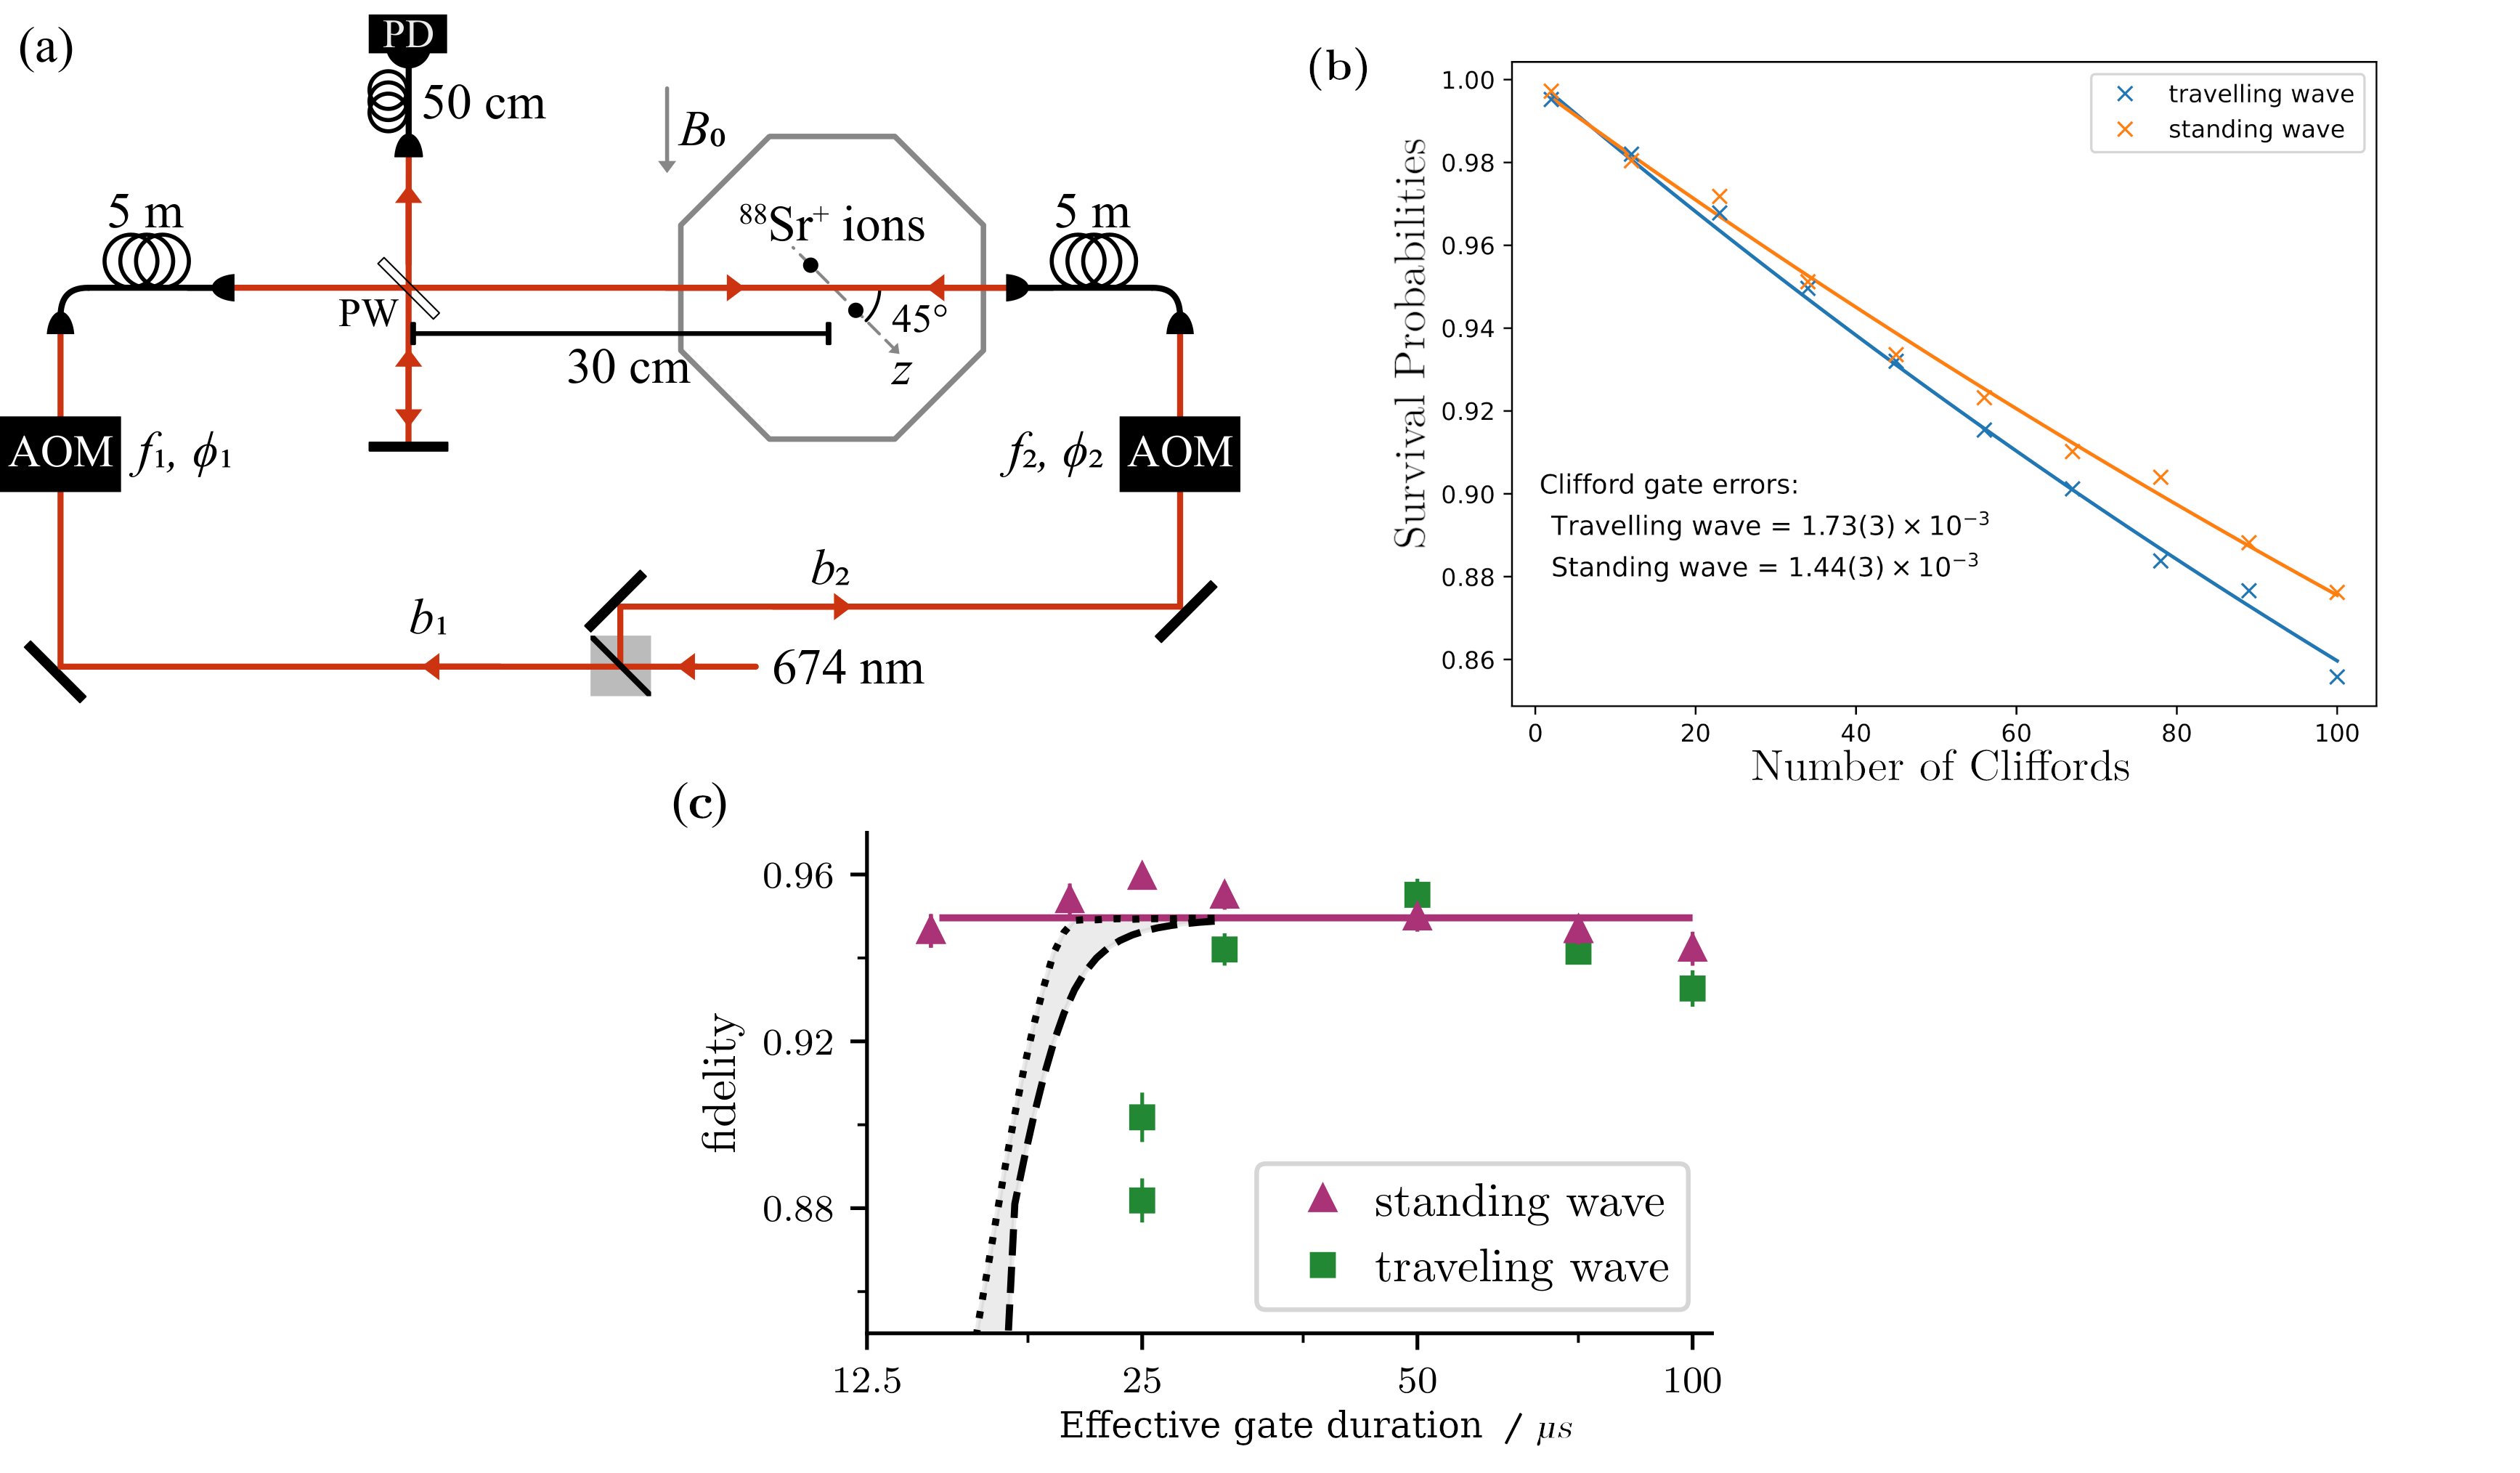
\includegraphics[width=\linewidth]{figures/cnulled_figs.png}
  \end{center}
  \caption{Carrier Null figs from [1] S. Saner and O. Băzăvan et al., `Breaking the
    entangling gate speed limit for trapped-ion qubits using a
    phase-stable standing wave'. arXiv, May 05, 2023.}

  \label{fig:cnull}
\end{figure}

    Here, we report experimental results of both standing wave (SW)
    single-qubit gates and SW Molmer-Sorensen
    entangling gates with the carrier term suppressed.\\
    These experiments were performed on our ``Blade'' apparatus which,
    although suitable for this proof-of-principle work, has hard
    limitations on what gate durations can be achieved due to
    available laser power and only global addressing of the ions.
    Section 3 will further discuss these limitations and the solution
    in form of a new ion trap apparatus.\\

    On ``Blade'' the SW is formed by two superimposed
    counter-propagating 674-nm beams and directed onto the ions at an
    angle of $45\degree$ to the ion chain. 674-nm light couples to
    the quadrupole qubit transition, 5S$_{1/2}$ $\Leftrightarrow$
    4D$_{5/2}$, in $^{88}$Sr$^+$.  The beams propagate in free-space
    and are phase-stabilized to ensure the SW is stationary with
    respect to the ion. Figure~\ref{fig:cnull}~(a) displays the path
    of the two counter-propagating beams. AOMs in both branches are
    used as switches, to apply sideband frequencies, and to control
    the phase of the beams.\\
    %% Light
    %% from each branch is picked off onto a fast photodetector forming an interference pattern to infer
    %% what phase corrections to feedback onto the AOMs. A slower
    %% secondary stabilization step is applied using the ion as a
    %% sensor. The ion is situated at what is believed to be a node of
    %% the SW and $\pi/2$ pulses on branch 1 and then immediately on
    %% branch 2 are applied.  This Ramsey like sequence gives a signal
    %% sensitive to the difference in phase between the two pulses, and
    %% may be used as an error signal to also feedback onto the control
    %% AOMs.\\

    %% are both utilized and
    %% benchmarked.

    %% An efficient $\pi$-pulse is achieved by setting the
    %% SW to be on resonance with the qubit transition and by placing a
    %% SW node at the ion.\\

    %% Figure~\ref{fig:cnull}~(b) shows the dependence of carrier coupling with phase of
    %% the SW seen by the ion. A monochromatic SW pulse on resonance with
    %% the qubit transition is applied. The pulse duration corresponds to
    %% a $\pi$-pulse at maximum carrier coupling, which occurs at the nodes
    %% of the SW.

    %% For an electric quadrupole transition, the maximum
    %% carrier coupling occurs at the maximum gradient of the electric
    %% field [9]. We can maximize the carrier coupling and minimize the
    %% sideband coupling, or vice versa, by selecting $\Delta\phi = \pi$ or $\Delta\phi = 0$.
    %% The transfer probability shown in Figure~\ref{fig:cnull}~(b) has a
    %% quartic dependence on $\Delta\phi$ near $\Delta\phi = \pi$ and a quadratic dependence at
    %% $\Delta\phi = 0$ [26]. When probing the suppressed motional sideband,
    %% Figure.~\ref{fig:cnull}~(b) left, we observe only features that are due to the
    %% off-resonant (by $\approx 1.2$~MHz) carrier coupling. By changing $\Delta\phi$ of
    %% the SW, we can realise any ratio between carrier and sideband
    %% coupling.\\

\subsection{Random Benchmarking}
%XX Add figure

    High fidelity unitary operations (gates) are essential for both
    near intermediate scale quantum computing and for reducing
    overheads in required physical qubits and operations in
    fault-tolerant schemes [x]. To evaluate whether the phase
    stability of our SW is sufficient for high fidelity gates, we
    employ randomized benchmarking (RBM) [32].  RBM consists of
    applying random combinations of a pre-chosen discrete set of gates
    to estimate an average error per gate.  We chose the single-qubit
    Clifford group as our set of gates to evaluate. The single-qubit
    Clifford group is the set of unitaries which map the Pauli
    matrices to one another through conjugation. This can be thought
    of as the complete set of rotations of the Bloch sphere such that
    all valid combinations of the axis
    $(x \rightarrow \{\pm x,~\pm y,~\pm z\}),~(y \rightarrow \{\pm x,~\pm y,~\pm z\}),~(z \rightarrow \{\pm x,~\pm y,~\pm z\})$
    are realized. There are 24 unitaries in this set. We followed the
    RBM protocol described in the Thesis [Amy] to evaluate our SW
    single-qubit gates. First the qubit is prepared in some known
    initial state, i.e. prepared in some chosen basis. A gate sequence
    is then applied which consists of multiple random Clifford gates
    followed by a final `inverting' Clifford such that the full
    sequence performs the Identity operation. The state is then
    measured in the same basis to find any deviations from the
    Identity being performed due to gate errors. This is repeated with
    the same preparation and sequence multiple times to calculate the
    probability that the Identity was performed - thus giving the
    sequence fidelity. These steps are repeated for many different
    random sequences with a range of sequence lengths. The sequence
    fidelity versus number of Clifford gates performed has now been
    found and a decay model is fitted to find the both the error per
    Clifford and the state preparation error.\\
    Using this method we compared the single-qubit gate errors when
    utilizing either standing or travelling waves. We obtained an
    error of $1.44(3) \times 10^{-3}$ and $1.73(3) \times 10^{-3}$ per
    Clifford gate for the SW and travelling single-qubit gates,
    respectively. Thus, use of the SW, and the added experimental
    complexity it entails, is not detrimental to single-qubit gate
    fidelity. Due to spin dephasing of our quadrupole qubit
    originating both from natural lifetime and external noise, we took
    care to ensure that the duty cycle and Rabi frequency of both SW
    and travelling wave RBM experiments were the same. \\

    %% ******************* Appendix? ****************
    %% * Could shift these derivations to the intro. \\
    %% First derivation of equation 1 of paper. \\
    %% By setting δ = 0 or δ = ±ωz, we can bring the carrier or sidebands
    %% into resonance, respectively. With ∆φ the SW has an additional
    %% degree of freedom compared to the TW: by setting 2 ∆φ = 0 we can
    %% drive the first sidebands while suppressing all even terms in the
    %% Lamb-Dicke expansion [26], including the carrier term. Conversely,
    %% if we set ∆φ = π we drive the carrier coupling and suppress all
    %% odd terms in the Lamb-Dicke expansion, including the first
    %% sidebands. \\

    %% The MS interaction requires two tones symmetrically detuned about the
    %% qubit resonance by δ ≈ ±ωz. To construct the Hamiltonian for a SW-MS
    %% interaction, we combine two monochromatic SWs as described by Eq. (1),
    %% resulting in the bichromatic SW interaction\\
    %% Equation 2 from paper\\

    %% where the phase ̃ φ =( ̃ φBD + ̃ φRD)/2 is now the mean optical phase
    %% between the blue- (BD) and the red- (RD) detuned SWs. Further, we
    %% assume that the BD and RD SWs are in phase at the position of the
    %% ion(s), i.e. ∆φBD = ∆φRD = ∆φ . The first term corresponds to a
    %% spin-dependent force (SDF) and the second term drives the carrier
    %% transition off-resonantly. Notably, these terms commute. Similar to
    %% the monochromatic SW, we can drive the motional coupling while
    %% suppressing the spurious carrier coupling by setting ∆φ = 0.\\

    %% ***********************************************


    %% We measure Rabi frequencies by scanning the SW pulse
    %% duration at the carrier resonance, for both ∆φ = π and ∆φ = 0. We
    %% observe this ratio to be 18, corresponding to a suppression 01234 2Ω/δ
    %% 0 20 40 60 80 Ω /2π (kHz) SDF traveling wave standing wave 024 2Ω/δ
    %% 0.0 0.5 1.0 Ω /(ηΩ) SDF FIG. 3. Spin-dependent force magnitude ΩSDF
    %% (normalized by ηΩ in the inset) versus 2Ω/δ , as measured for a single
    %% ion with η = 0.05. We extract ΩSDF by applying a conventional
    %% bichromatic TW field (squares) or a bichromatic SW field (triangles),
    %% for variable durations. The solid lines show the analytical
    %% dependence; as predicted by the theory and shown explicitly in the
    %% inset, the TW coupling follows the Bessel functions (|J0 + J2|), while
    %% the SW coupling remains constant [34]. of 25 dB between maximal and
    %% minimal carrier coupling. This suppression is consistent with the
    %% measured interferometric stability and the residual power imbalance
    %% between b1 and b2.\\


    %% This has a lot of experimental detail. Maybe too much for the report.\\
    %% Next, we experimentally investigate the saturation effect caused
    %% by the non-commuting carrier coupling [Eq. (3)] when generating an
    %% SDF with a bichromatic TW, and compare it to the SDF generated by
    %% a bichromatic SW. To create the TW bichromatic field, we apply two
    %% tones to the AOM in b1, while for the SW we apply the same two
    %% tones in both beams, b1 and b2. These tones are symmetrically
    %% detuned by δ ≈ ±ωz from the qubit resonance. This results in an
    %% SDF on the axial mode (ωz/2π ≈ 1.2 MHz) of a single ion. We
    %% extract its coupling strength ΩSDF(Ω, δ ) by applying the SDF for
    %% variable durations [29]. We used an adiabatic ramp duration of 3.6
    %% μs for these measurements [33]. For the TW, we observe a coupling
    %% that scales with the expected Bessel function dependence |J0(2Ω/δ
    %% ) + J2(2Ω/δ )| [Eq. (4), Fig. 3]. Hence, when using the TW, there
    %% exists a maximum achievable interaction strength that imposes a
    %% speed limit on the interaction regardless of the available laser
    %% power. This limit is caused by the increasingly strong offresonant
    %% non-commuting carrier excitation and not by technical aspects such
    %% as pulse shaping. For the SW, we demonstrate that no such
    %% speed-limit exists. We place the ion at the maximum intensity of
    %% both the red- and the blue-detuned SWs [26] and observe that the
    %% interaction magnitude [34] increases linearly with Ω (Fig. 3).\\

\subsection{Standing wave Molmer-Sorensen}

    To explore two-qubit entangling gates we implemented an MS-type scheme
    with a bichromatic SW instead of the conventional
    bichromatic TW. The bichromatic field is created by applying two
    tones to the AOMs in Figure~\ref{fig:cnull}~(a). As with the TW MS-scheme, these
    tones are symmetrically detuned by $\delta \approx \pm(\omega_z + \delta_g) $ from the
    qubit resonance. Here $\omega_z$ 
    is the axial mode frequency of our trapped single ion,
    $\omega_z = 2\pi\times 1.2$~MHz, and $\delta_g$ is some further detuning
    from these sidebands. To selectively couple to the sidebands, and
    hence suppress the carrier term, the ion spacing is adjusted to
    place them both on antinodes of the bichromatic SWs.\\
    We performed TW and SW two-qubit entangling gates on the axial
    in-phase mode and optimize the experimental parameters to maximize
    the Bell-state fidelity for a fixed gate duration. In both cases,
    we use a ramp duration of 10 $\mu$s to minimize coupling to the other
    motional modes [33]. In Figure~\ref{fig:cnull}~(c), we show the two-qubit fidelities
    achieved with the two schemes as a function of the effective gate
    duration ($2\pi/\delta_g$, where $\delta_g = \delta - \omega_z$) [37]. For slower gates,
    the fidelity of the SW-MS is comparable with that of the
    TW-MS. For faster entangling gates, the fidelity of the TW-MS
    degrades rapidly as expected due to the carriers presence. In contrast, the fidelity for the SW-MS is
    consistent with $\approx 0.95$ over the entire available power range,
    showing that we have eliminated the limit arising from the carrier
    coupling. The shortest SW-MS gate was 15 $\mu$s, limited by the
    available total power of 29 mW. \\

    As gate duration is inversely proportional to Rabi frequency, we
    can further push the speed of these gates using greater
    intensities of light at the ions. This can be achieved by more
    powerful lasers or by focusing the beams down to tighter waists at
    the ions locations. To explore these faster gates a new apparatus
    has been designed and is being constructed that will feature both
    these improvements and will allow exploration of these gates in
    many ion crystals. A description and progress report of this
    system is described in the following section.\\

    %% In conclusion, we implemented single- and two-qubit operations for
    %% trapped-ion qubits using a phase-stabilized SW. Two
    %% counter-propagating beams create the SW, whose relative phase ∆φ at
    %% the ion position is stable to ≈ λ /100. This enabled us to tune the
    %% ratio of the field intensity and gradient that the ions experience,
    %% which sets the relative strengths of the sideband and carrier
    %% interactions. We use this new degree of control to suppress the
    %% unwanted off-resonant carrier coupling (by a factor of 18), while
    %% coherently enhancing the motional coupling during two-qubit gates. We
    %% show theoretically and experimentally that the non-commuting carrier
    %% term imposes a limit on the speed of conventional TW-MS gates, which
    %% were avoided using the SW-MS interaction. These optical phase control
    %% techniques could also be applied in the previous Raman-based scheme
    %% [16], where they could mitigate squeezing terms, which were the
    %% leading error source; we note that for the SW-MS those terms are
    %% inherently suppressed. Our work shows a clear path towards entangling
    %% gates with durations comparable to the motional period of the ions (∼
    %% 1 μs or shorter) at wavelengths that are amenable to largescale chip
    %% integration using standard integrated optics [3840] and without the
    %% technical challenges of using high-power blue Raman beams [16], pulsed
    %% lasers [41, 42] or Rydberg schemes [43].\\

%}}}

%Experimental Details {{{
\section{Experimental Apparatus}

The technical complexity of ion trapping experiments may be reduced to
solving two problems: controlling the state of the ion (both internal
and motional); and controlling the ion's surrounding environment.
Our ion trap experiments consist of: an atomic source, a trap, a
vacuum system encasing these, external magnetic field coils, and
lasers for ionization, cooling, repumping, state preparation, coherent
control and readout.\\
%% As with all ventures in experimental physics, as technologies mature, so
%% too do the capabilities and scope of our apparatus.
Here we describe both the older generation apparatus, referred to as ``Blade'',
where the proof-of-principle fast gate schemes have been tested[ref
  cnull, ref vera], and the new proposed system known as
``FastGates'', which solves critical limitations for further exploring
fast entanglement.


\begin{table}[h!]
\begin{center}
\begin{tabular}{ c|c c c c }
  Trap & $d$ / $\mu$m & $\omega_{ax}, \omega_{rad}$ / ($2\pi$MHz) & $\dot{\bar{n}} / qs^{-1}$ & Trap depth / meV \\ 
  \hline
  Blade  & 500 & 1.9, 4 & 75 & 1000 \\
  HOA2  & 68 & 1.8, 2.5 & 2000 & 150 \\
  NPL  & 250 & ~1.6*, 5.0* & <100~ & ~400* 
\end{tabular}
\caption{Comparison of different trap types at typical operating
  parameters. Blade is a macro blade style trap, HOA2 is a surface
  style trap, and NPL is a microfabricated 3D trap. $d$ is the
  ion-electrode distance, $\omega$ are the motional mode frequencies
  for one ion, and $\dot{\bar{n}}$ is the heating rate in quanta per
  second. NPL starred values are from simulation. Values for Blade and
  HOA2 came from [Vera, Amy Thesiss] and [DPN, Beth Thesiss]
  respectively. }

%% Characterization of a High-Optical-Access surface trap optimized for quantum information processing Peter Maunz, Craig R. Clark, Raymond Haltli, Andrew Hollowell, Jonathan Mizrahi, John Rembetski, Paul Resnick, Jonathan D. Sterk, Daniel L. Stick, Boyan Tabakov, and Matthew G. Blain Sandia National Laboratories  
\end{center}
\label{table:trap}
\end{table}

\begin{figure}
  \begin{center}
   \noindent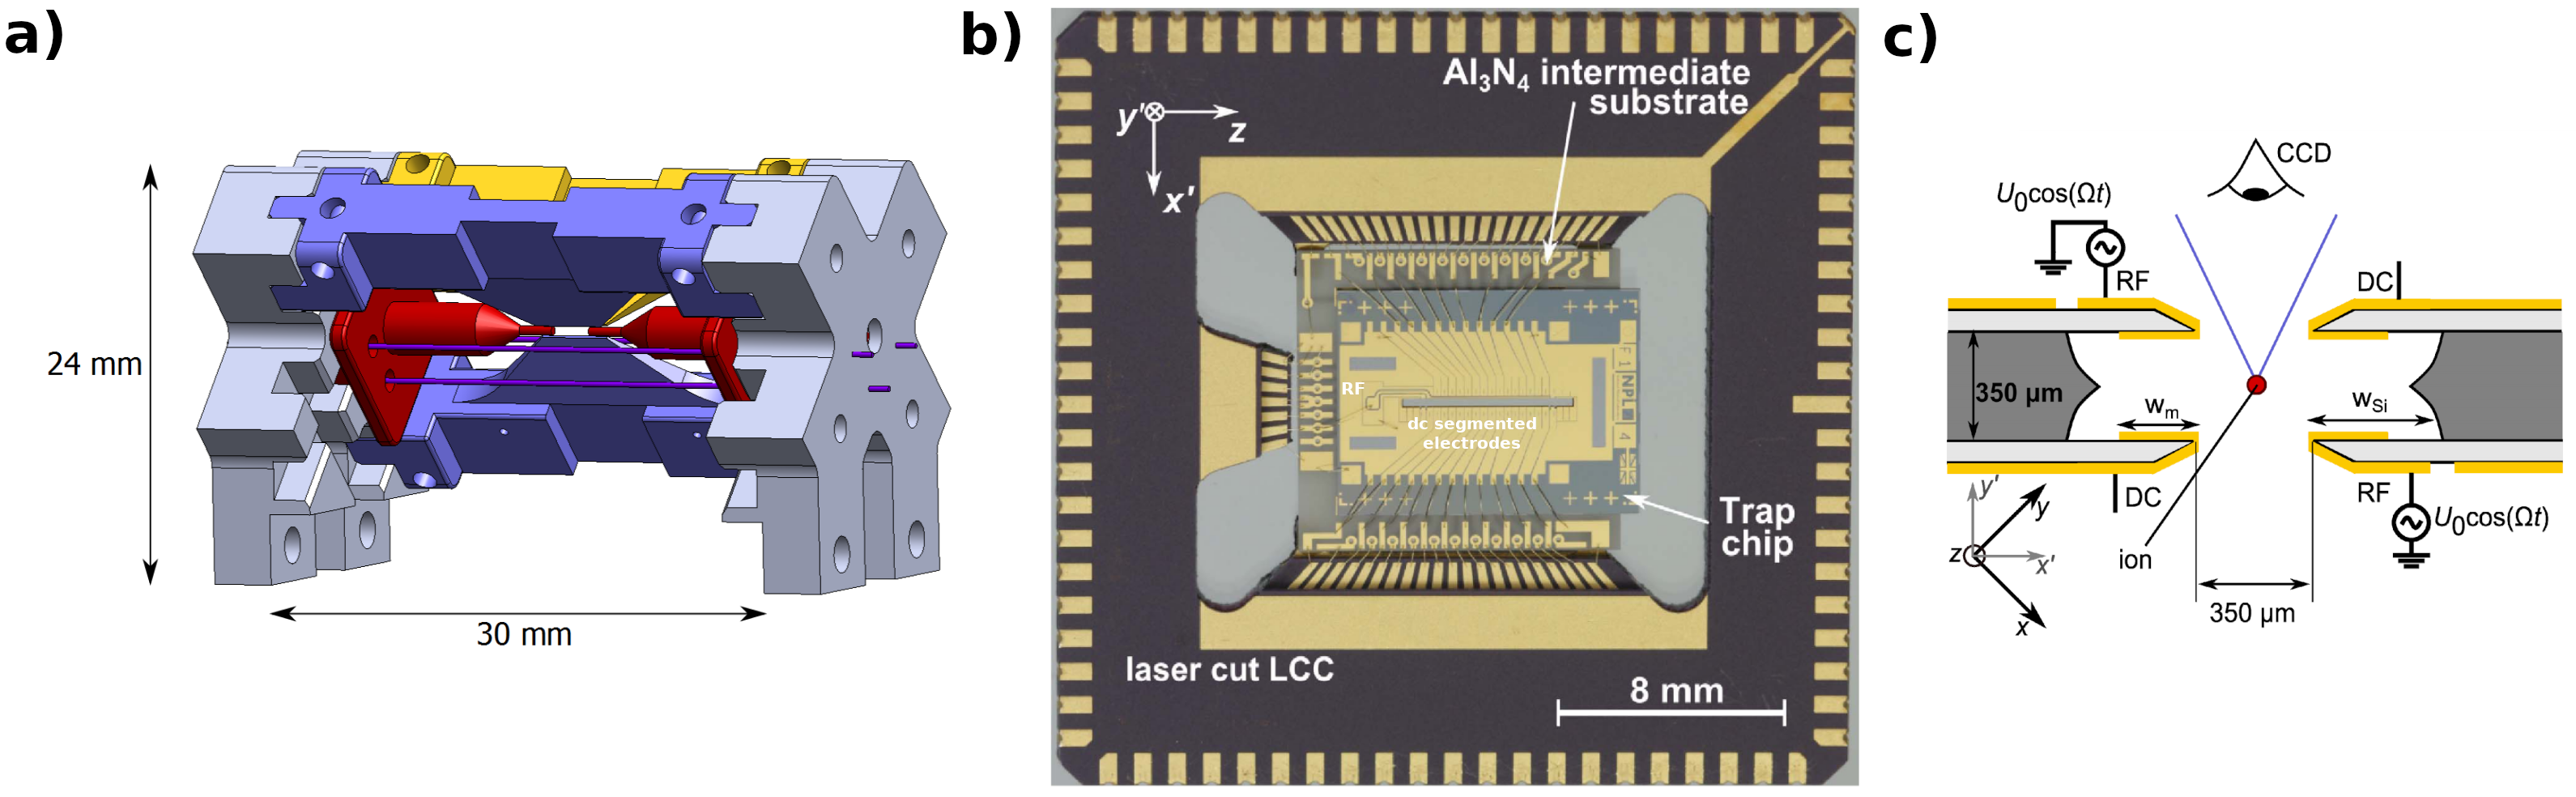
\includegraphics[width=\linewidth]{figures/trap_comp.png}
  \end{center}
  \caption{\textbf{a)} Blade trap used for carrier nulling results. In
    blue are the RF blades providing the radial pseudopotential whilst
    in red are the DC end caps providing the axial
    potential. \textbf{b)} NPL trap being used in the FastGates
    experiment. This is a microfabricated, segmented, multilayer
    trap. \textbf{c)} A cross sectional view of the NPL trap showing
    the RF and DC electrode positions.
    Figures from [S. R. Woodrow]
    %%     Linear Paul trap design for high-fidelity ,
    %% scalable quantum information processing. Master’s thesis, University
    %% of Oxford, 2015
    and [K. Choonee].
    %%   G. Wilpers, and A. G. Sinclair,
    %% ‘Silicon microfabricated linear segmented ion traps for quantum
    %% technologies’, in 2017 19th International Conference on Solid-State
    %% Sensors, Actuators and Microsystems (TRANSDUCERS), Jun. 2017,
    %% pp. 615–618. doi: 10.1109/TRANSDUCERS.2017.7994124.
  }

  \label{fig:trap}
\end{figure}

\subsection{Ion}
We use alkali like ions (Group 2 elements) due to their single outer electron with Hydrogen-like energy levels. For ``FastGates'' we will use $^{40}$Ca$^+$

First let us consider the \textsuperscript{40}Ca\textsuperscript{+} energy
level structure, figure X. The \textsuperscript{40}Ca\textsuperscript{+} has
no nuclear spin and is hydrogen like with only one electron in the outer shell
giving a (relatively) simple level structure. An external magnetic
field of $5$ G is applied to split the levels via the Zeeman effect. The relevant
laser transitions for our planned ion trap experiment have been marked
and their purpose and construction shall be discussed below.\\

The natural lifetime of the metastable
3D\textsubscript{5/2} is around 1.1 s XrefBarton, giving a favorable
fundamental limit of coherence time for our chosen qubit.
This natural lifetime leads to a narrow 4S\textsubscript{1/2} $\Leftrightarrow$
3D\textsubscript{5/2} transition linewidth $\Gamma < 1$~Hz, and so
demands the use of a narrow linewidth laser, which is discussed in the \textit{Laser} subsection.

\textsuperscript{40}Ca\textsuperscript{+} was chosen for zero nuclear
spin and therefore simple energy level structure. However we now
cannot utilize hyperfine structure to find ``clock'' qubits which are
insensitive to magnetic field fluctuations and must instead remove
magnetic field noise from the environment. To suppress this noise 
we place the vacuum chamber within a box constructed from two layers
of 3mm thick MuMetal [ref]. The shielding was shown to suppress the
background field by a factor of 500 at its center. XXHow does this
effect noise affecting decoherence? and shorten paragraph.

\subsection{Trap}
%% As mentioned in section 1, the overall system we desire is an internal electronic state of the ion coupled to its motion.
%% Our ion in this case being a Hydrogen-like ion, and the
%% spring being the harmonic motion of the ions within the trapping
%% potential.

To create the trapping potentials we use linear
Paul traps, a schematic of such is shown in
Figure~\ref{fig:trap}~(a). As explained by Earnshaw's theorem,
$(\nabla^2 V = 0),$
a stable stationary point in 3D can not be realized using only static
electric potentials, $V$, as if the potential is confining in two
dimensions, it will be anticonfining in the third. Therefore, to
achieve stable trapping an oscillating field must be utilized to create a pseudopotential.
%Include pseudopot eqn?
A Paul trap achieves this through an oscillating RF electric field
providing radial confinement and a static field to create axial
confinement.
%% There are various popular geometries for realizing a Paul
%% trap: macroscopic 3D Blade traps; surface traps; and microfabricated
%% segmented 3D traps.
A Blade trap, Figure~\ref{fig:trap}~(a), as is used in the ``Blade''
apparatus, has axial confinement created by DC end caps and radial
confinement by supplying an oscillating RF voltage to the blades. In
``Blade'' the ion endcap distance is $1.15$~mm, and ion-blade distance
is $0.5$~mm. Typical operating frequency for the RF electrodes of the
``Blade'' trap are $28.0133$ MHz leading to an axial ion frequency of
$1.860$ MHz and radial frequencies of $4.077$ MHz and $4.341$
MHz.\\ Recently, the surface style linear Paul trap has gained
popularity due to the maturity of chip fabrication technologies[ref]
and the potential route to scalability this offers. In the surface
trap, the 3D blade and endcap geometry of the ``macro'' trap is
effectively projected onto a 2D surface. The stable point of such a
trap is typically on the order of $50$ $\mu$m from the chip
surface. The ease of fabrication of surface traps has allowed the
creation of complex multizone devices with many DC electrodes.  These
multizone traps enable the shuttling of ions, a requirement for
Quantum CCD type architectures [ref]. However, this surface style
geometry greatly reduces the depth of the trapping potential and the
close proximity of the surface to the ion is a large contributor to
anomalous heating[ref]. Values for a widely used surface style trap, HOA2
[ref], are summarised in table~\ref{table:trap}.\\
A microfabricated 3D trap [See et al and Wilpers 2012], as will be
used in the ``FastGates'' apparatus, brings together the advantages of
chip fabrication as well as low heating rates and high trapping
depths of a 3D style trap with greater ion-surface distances. This is
achieved by a multilayer chip as shown in Figure~\ref{fig:trap}~(b,
c). The radial trapping is provided by RF rails on opposite diagonals
of the slit whilst axial trapping may be realized by DC
electrodes. The ion-surface distance is now of the order $250$ $\mu$m and
the heating rates have been shown to be $< 100$~q/s [ref]. 
%% The 3D confining potential
%% leads to motion of the ions following the Hamiltonian

%% $$ H = \sum_{i=1}^N \frac{m}{2}(w_x^2x_i^2 + w_y^2y_i^2 + w_z^2z_i^2 + \frac{|p_i|^2}{m^2}) + \sum_{i=1}^N\sum_{j>i}\frac{e^2}{4\pi\epsilon_0|r_i - r_j|}$$,

%% where $w_v$ are the mode frequencies in the three dimensional
%% coordinated.
%% We define $z$ to be the axial direction of the trap and
%% typically assume $w_z$ < $w_x$, $w_y$ to allow a 1D ion crystal to
%% lie along the axial direction of the trap.
We aim for an axial ion
separation of around $5$~$\mu$m which, for $^{40}Ca^{+}$ ions means a
trapping potential of $\omega_z \approx 2\pi \cdot 1.6$~MHz. This ion
separation was chosen to reduce the cross talk between ions when
singly addressed (see section X).\\
We are targeting approximately $5$~MHz for our radial frequencies, as
we shall use radial addressing for two-qubit entangling gates. The choice
of this higher frequency is motivated by several factors. The Doppler
cooling limit ($\overline{n} = \Gamma/\omega$, where $\Gamma$ is the
transition linewidth and $\omega$ is the frequency of the cooled mode) 
inversely scales with the mode frequency. Consequently, higher
mode frequencies result in lower temperatures following initial
cooling. Additionally, a higher center-of-mass radial mode enables
greater frequency separation of radial modes in a multi-ion crystal,
which allow for greater selectivity of participating modes. \\
Using the pseudopotential approximation for the confining field, we can find a
trapping frequency in one radial direction $\omega_p$
$$\omega_p = \frac{e\alpha V_{RF}}{\sqrt{2}\Omega_{RF}M\rho^2},$$
where $\alpha$ is a factor of order unity given by the geometry of the trap, $V_{RF}$ and $\Omega_{RF}$ are the voltage and frequency provided to the RF-electrode, $M$ is the mass of the ion, and $\rho$ is the ion-RF electrode separation.
Applying some DC voltage on the axial electrodes leads to axial confinement with frequency $\omega_{ax}$, but must defocus the radial confinements as the total curvature of the pseudopotential must remain constant,
$$\omega_{rad} = \sqrt{\omega_p^2 - \omega_{ax}^2/2}.$$
Unlike the macroscopic blade trap, the NPL trap focuses one of
the radial modes and defocuses the other when the DC electrodes are
increased due to the ``cross'' arrangement of DC and RF electrodes,
Figure~\ref{fig:trap}~(c),
$$\omega_{rad\pm} = \sqrt{\omega_p^2 - (1\mp\beta)\omega_{ax}^2/2},$$
where $\beta$ is some factor due to the geometry of this cross arrangement. From simulation $\beta > 1$ for $\Omega_{RF} = 2\pi\cdot 23$~MHz and $V_{RF} = 200$~V and so one radial mode increases with DC voltage applied and one decreases as can be seen in figureX.
\begin{table}[h!]
\begin{center}
\begin{tabular}{ c|c c c c c c }
   & $V_{RF}$ / V & $\Omega_{RF}$ / ($2\pi\cdot$MHz)& $V_{DC}$ / V & $\omega_{ax}$ / ($2\pi\cdot$MHz) & $\omega_{rad}$ / ($2\pi\cdot$MHz) & q \\ 
  \hline
  Experiment  & 200 & 23 & -7 & 1.6 & 4.9 & 0.61 \\
  Loading  & 100 & 23 & -2 & 0.8 & 2.0 & 0.25 \\
\end{tabular}
\caption{ Simulated parameters for both ``Experiment'' and ``Loading'' settings \textsuperscript{40}Ca\textsuperscript{+} with the NPL trap.
  }
\end{center}
\label{table:freqs}
\end{table}
A possible set of parameters to achieve $\omega_{ax} = 2\pi \cdot
1.6$~MHz and $\omega_{rad+} = 2\pi \cdot 4.9$~MHz can be seen on the
``Experiment'' trapping in table~\ref{table:freqs}.  From Mathiu
equations, stable trapping exists for $q < 0.9$[ref], where
$q=2\sqrt(2)\omega/\Omega_{RF}$, however convenient trapping of hot
ions requires $q$ to be as low as possible. To satisfy this
requirement a ``Loading'' setting (with parameters in
table~\ref{table:freqs}) may be used with $q = 0.25$ and then the
$V_{RF}$ ramped to the ``Experiment'' trapping for high radial mode
frequencies.

\subsection{Laser systems}

Lasers are a key tool for creating the highly localised, strong
electric field amplitudes and gradients needed to drive both carrier
and sideband transitions of the trapped ion.\\


\begin{figure}
  \begin{center}
   \noindent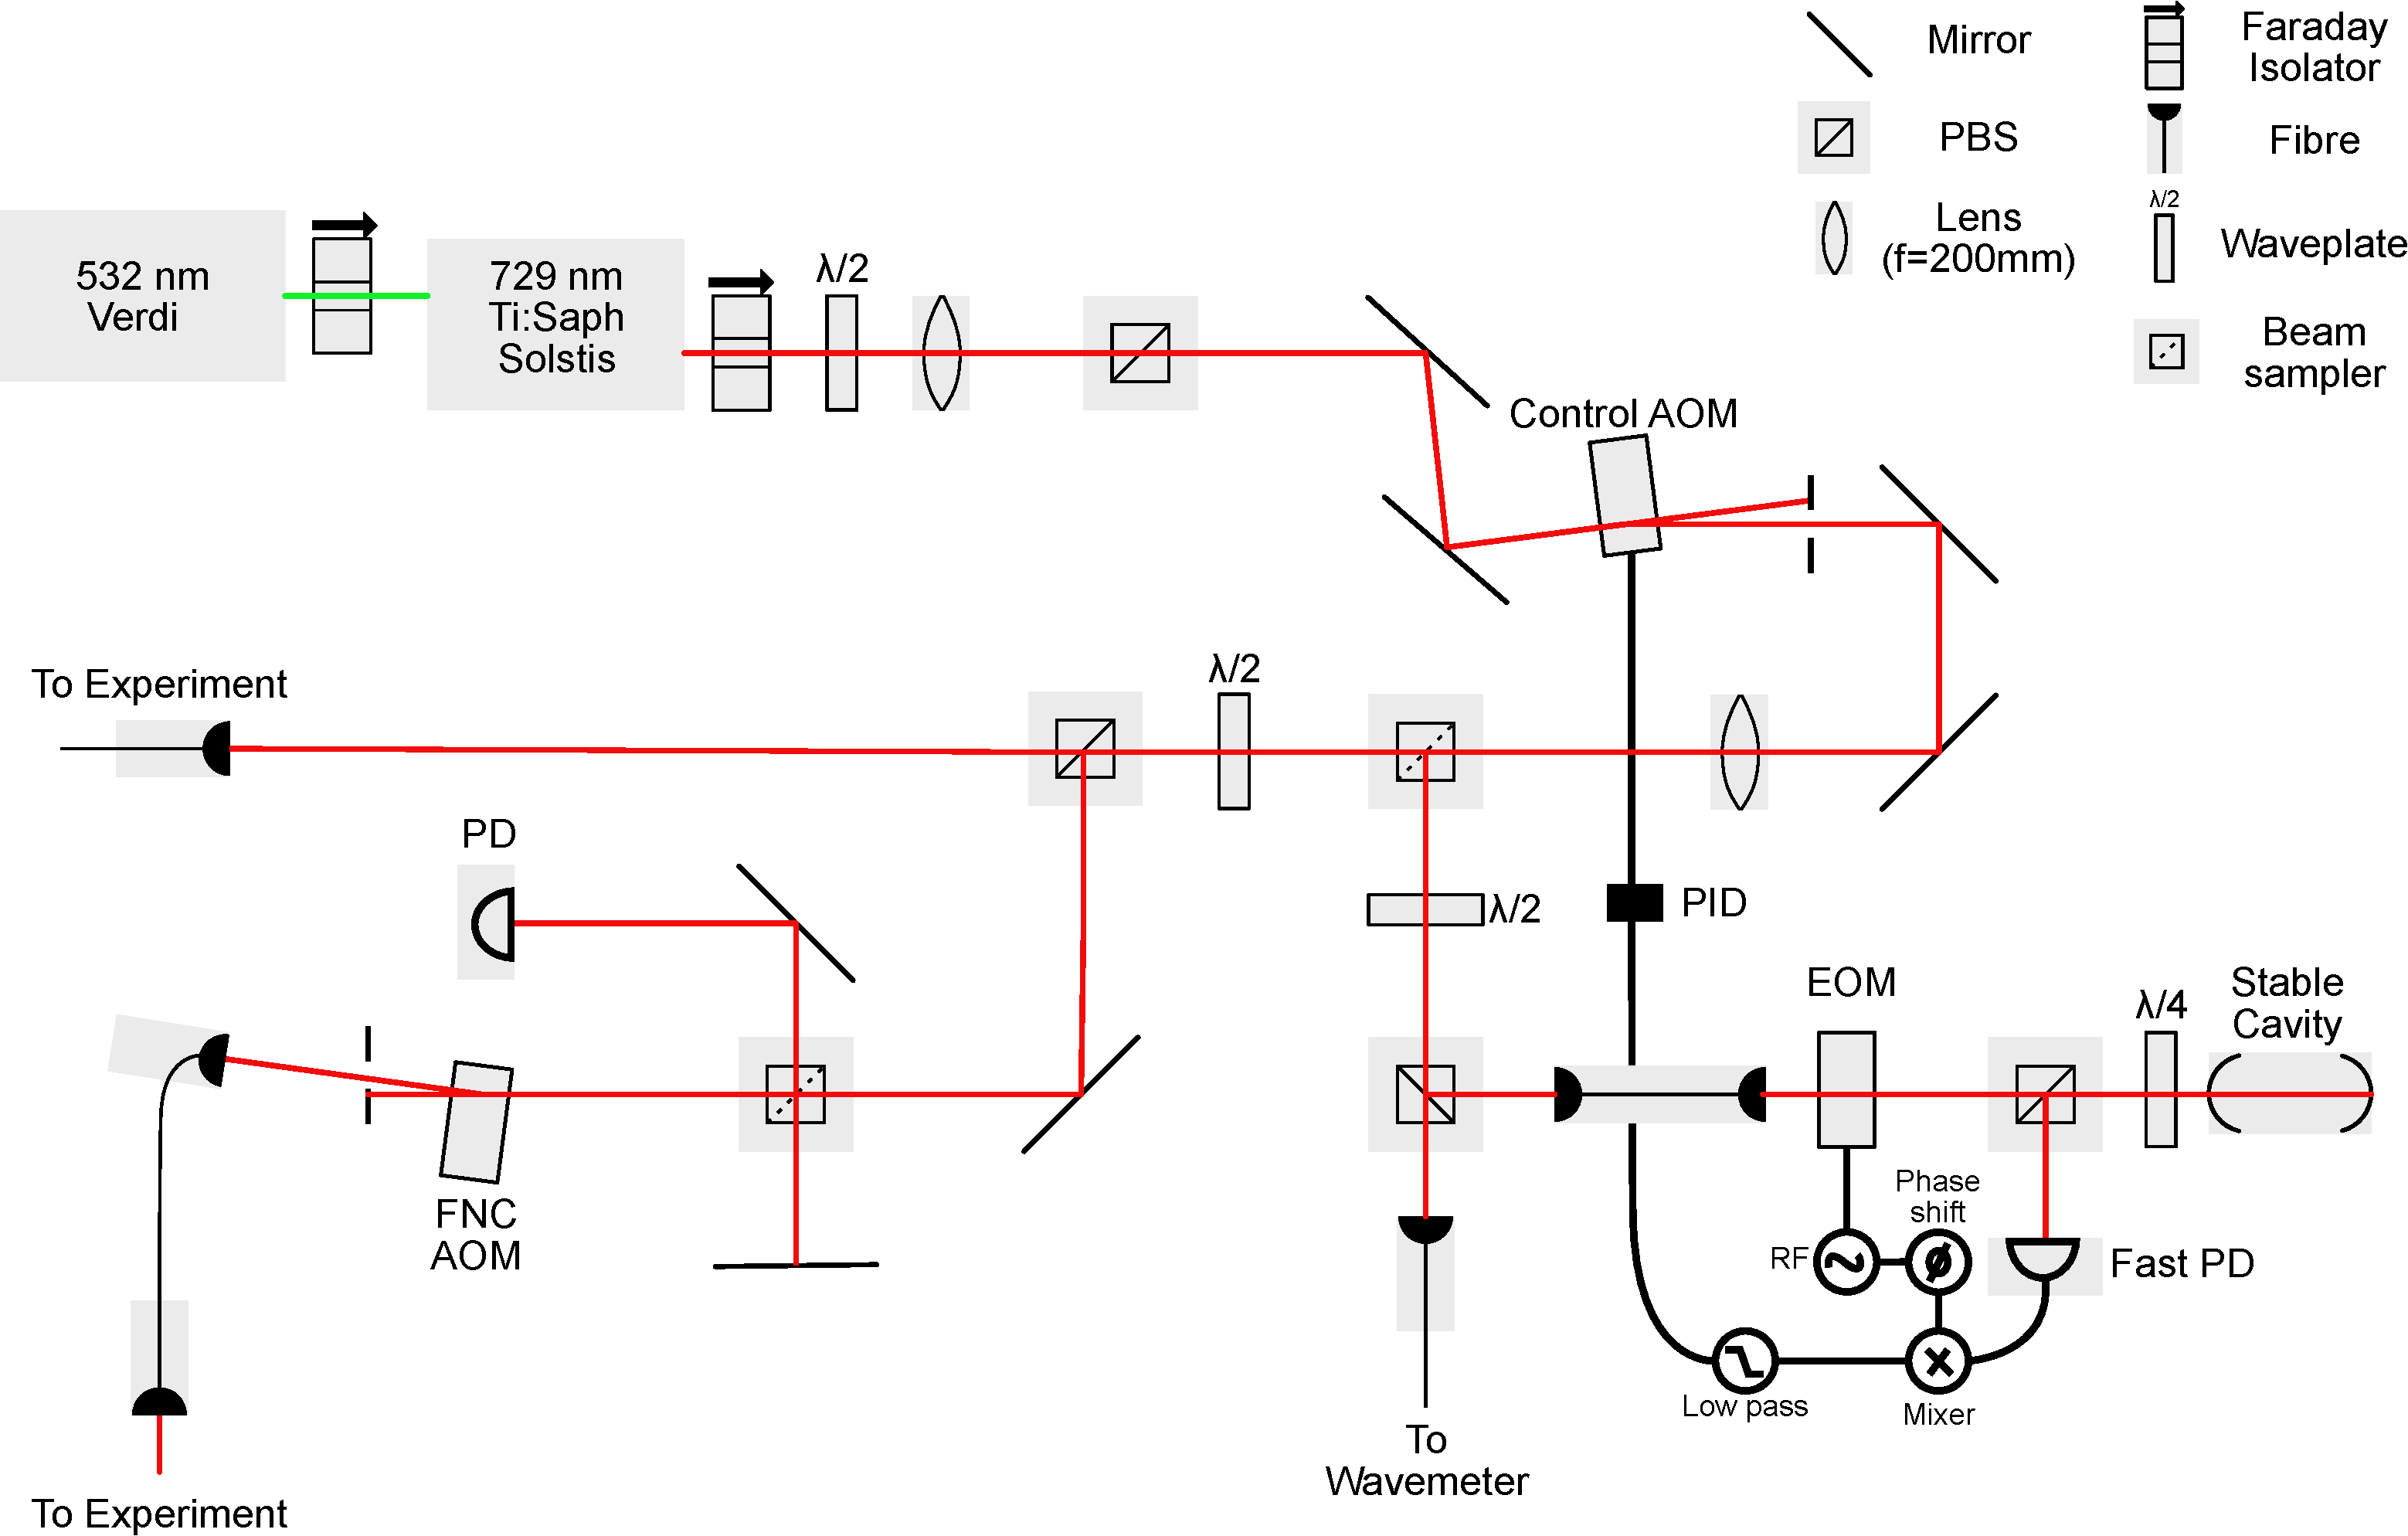
\includegraphics[width=\linewidth]{figures/729_path_small.pdf}
  \end{center}
  \caption{729-nm system}
  \label{fig:729}
\end{figure}

As shown in FigureX we will use the levels
4S\textsubscript{1/2} to 3D\textsubscript{5/2} with a 729-nm
quadrupole transition to define our qubit. Therefore the 729-nm laser
is used to implement single- and multi-qubit gates. We also use this
transition, after Doppler cooling, for resolved sideband cooling to
bring the motional mode close to its ground state.

This laser must be narrow linewidth ($\Gamma < 1$~Hz), and for fast gates we require
large electric-field intensities at the ion to drive sideband transitions due to a low
Lamb-Dicke factor for the 729-nm transition[ref].
Pumped Ti:Saph laser systems have been shown to be both relatively
high power and narrow linewidth, making them suitable for our
experiment.

We pump an M2 Solstis Ti:Saph with 15 W of 532-nm light from a Verdi
system to produce around 4W of 729-nm light.  A schematic of the
729-nm system being built is shown in Figure~\ref{fig:729}. The
frequency is
stabilized by the Pound-Drever-Hall (PDH) technique with a high
finesse cavity. PDH locking requires taking the laser light and
applying two sidebands via an electro-optical modulator (EOM). This
phase modulated light is then directed onto a stable cavity and a
reflected signal is directed onto a fast photodetector. The reflection
from the cavity consists of the interference between the carrier and
the sidebands which have been respectively altered by the cavity
transfer function. The photodetector signal is mixed down with the
same oscillator signal as provided to the EOM but delayed by some chosen
phase, and finally low pass filtered to produce a signal for use as
the error signal in the servo loop.  This error gives a measure for
how far the carrier frequency is from the stable cavity resonant
frequency and is used for feedback onto the control AOM situated after
the Solstis.

Some of the 729-nm light is picked off and sent to a wavemeter to
monitor the frequency. However, the majority is coupled to two output
fibres for our experiment and another within the group. We transport
the 729-nm light from a dedicated laser lab to a room containing the
trap apparatus by a 10~m single mode polarization maintaining.  To
remove the phase noise introduced by mechanical and thermal effects in
the fibre we implement fibre noise cancellation[ref].



%% Trial of Verdi C unsuccesful so far not achieving stable lasing with
%% solstis.
%% Improvements over Blade:
%% - 729 more convenient Ti:Saph freq -> Higher power, low noise
%% - access parallel to radial mode, Blade is 45 deg -> High Lamb Dicke
%% factor
%% - 729 more convenient for putting in fibre -> low charging

%% The remaining transitions utilize Toptica diode lasers with PDH
%% locking on a stable cavity from Stable Laser Systems. They consist of:
%% \begin{itemize}
%% \item 393-nm and 423-nm - for two step photoionization with isotope selectivity
%% \item 397-nm - for Doppler cooling and fluorescent readout.
%% \item 854-nm and 866-nm - for repumping any lost population from the P to the D states.
%% \end{itemize}


\subsection{Inside the vacuum}

\begin{figure}
  \begin{center}
   \noindent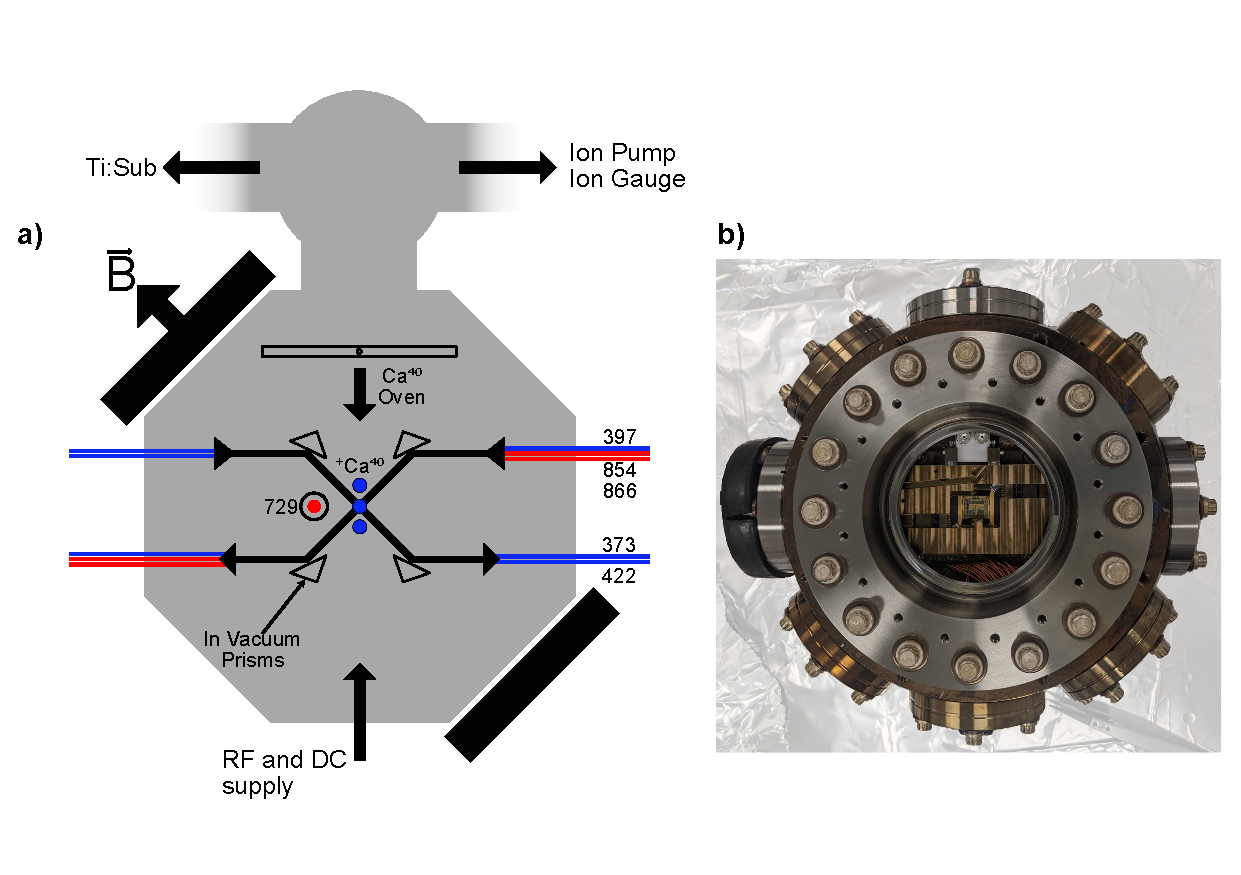
\includegraphics[width=\linewidth]{figures/vacuum_can.pdf}
  \end{center}
  \caption{Vacuum can}
  \label{fig:can}
\end{figure}

Here, we describe the instrumentation required, and being
constructed, for decoupling the ion from any unwanted external
environments. Our primary tools for this are working under Ultra High
Vacuum (UHV) and surrounding the vacuum system with electromagnetic
shielding. Inside the vacuum system we aim for a residual pressure of
less than $10^{-11}$ mbar. To reach this pressure, we must take
care in material choice and thoroughly clean and bake all material
within the vacuum system (a useful summary of tactics can be found in [ref, Jochen?]).

A schematic and photograph of the vacuum system can be seen in
Figure~\ref{fig:can}. The system consists of an octagonal experimental
chamber connected to an Ion pump, Ion Gauge and Ti:Sub pump. For
optical access we have Dual CF100 viewports coated for 397-nm and
729-nm as well as two CF40 viewports coated for 397-nm, 422-nm,
729-nm, 854-nm and 866-nm.

We use in vacuum prisms to direct light onto the ions located within
the slit of the NPL trap as there is no visibility of the ions from
the side CF40 viewports and the high NA lens needed for single
addressing obstructs the CF100 entry.

We use an electrical feedthrough on a CF40 flange to supply our trap
chip with both DC and RF voltages. As the DC cables run within close
proximity to the RF supply, electrical pick up is a potential issue
within our DC lines. We mitigate this through a low pass filter board
within close proximity of the trap chip.
%% We implement a ``trap
%% stack'', as can be seen in the photograph of Figure~\ref{fig:can}, within the vacuum chamber consisting of the
%% trap chip, the outer chip carrier, an interposer, and the filter PCB.


\subsection{Single Addressing}

\begin{center}
Still Under Construction \\
\end{center}
\hrule\vspace{1em}

\begin{figure}
  \begin{center}
   \noindent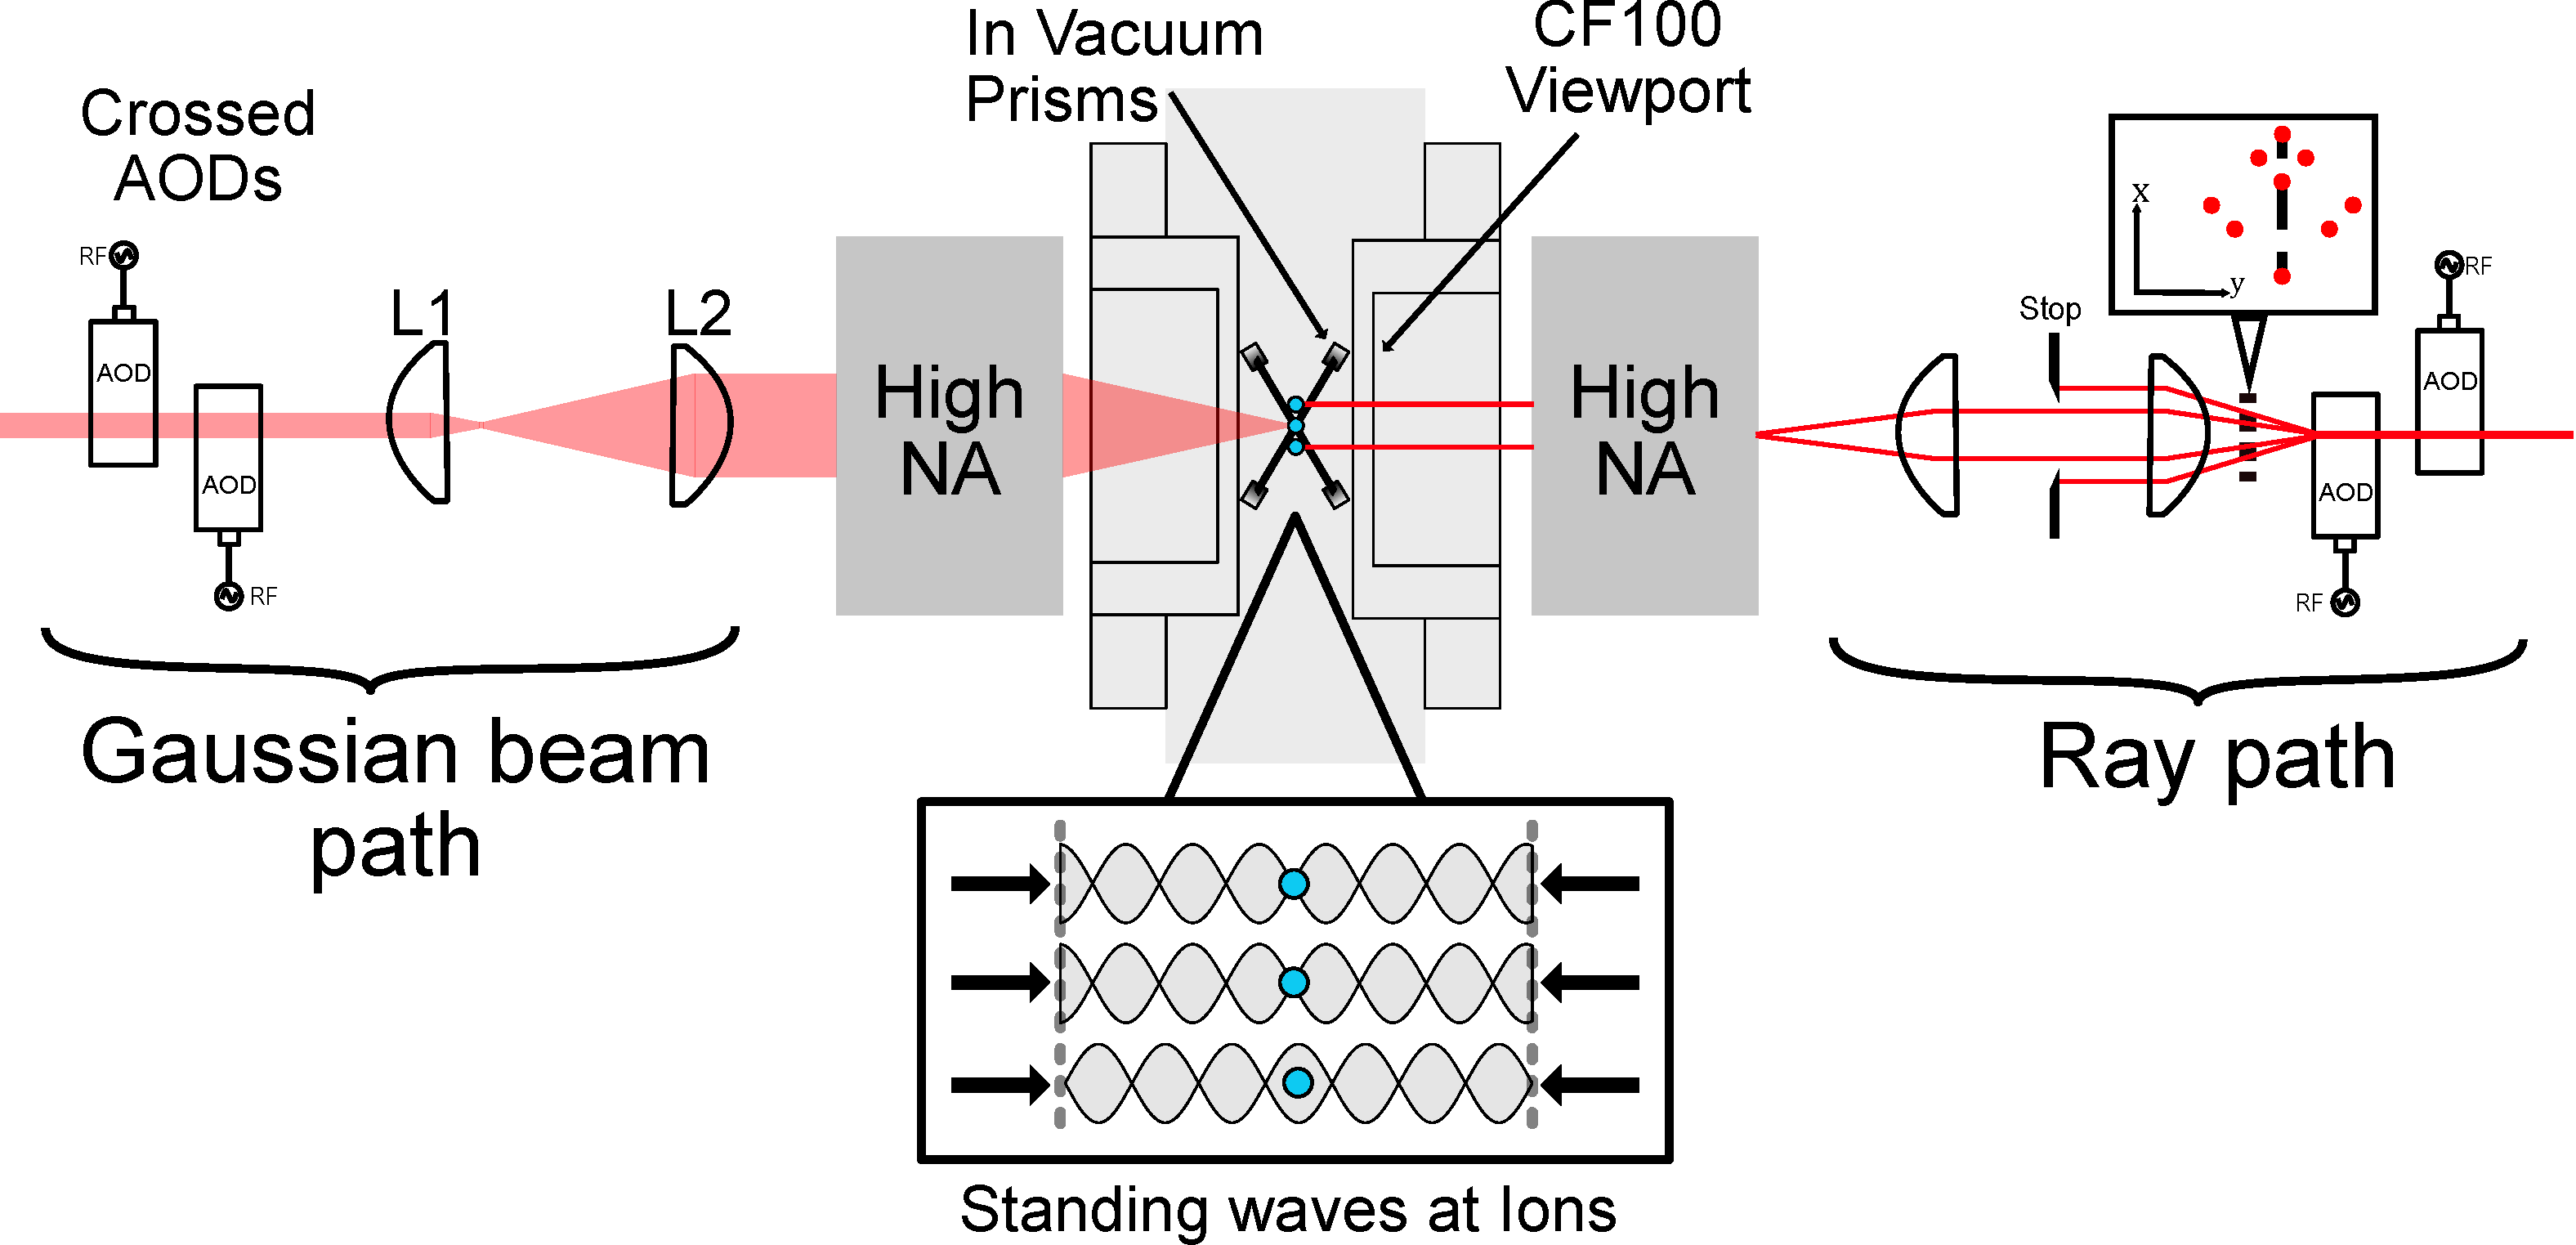
\includegraphics[width=\linewidth]{figures/vac_can_AOD_small.pdf}
  \end{center}
  \caption{Single addressing system}
  \label{fig:AOD}
\end{figure}

729 High NA (0.6) lens we can achieve waist radius of < 1 um.  With
our axial trap freq of $1.6$~MHz we get ion spacing of ~ 5um.  Using AOD
system we can traverse this ion chain.
\begin{itemize}
\item Description of lens system from AOD to ions.
\item Description on the mechanism on how AOD works (this is the same
  as an AOM) (Probably skip this).
\item Comparison between this and a fixed waveguide array.
AOD have extra programmable control than waveguides which is
excellent as we are in an exploratory regime where we may want to
alter ion spacing/Dont want to use quartic potentials to make ions
evenly spaced.
There is minimal path length difference compared to waveguide which is
ideal as we can stabilise at some central frequency and should be
stable at all ion locations.
\item We will use a crossed AOD design so that we have no overall frequency
shift as we scan along the ion chain.
\item Compact design to fit beam path within MuMetal box. (Probably skip this).
\item Using two RF freq so that we can address two ions at the same
time. Comes at cost of power due to cross terms.
\end{itemize}

%% However addressing multiple ions at the same time comes at the cost of
%% photon freq cross terms i.e. spots that we dont want that are off
%% plane to our ions. This has two bad effects: Can get crosstalk to
%% other ions on the chain and lose power in our 729 system. First effect
%% we can mitigate by putting AOD at a > 45 deg angle (60 deg?) this
%% pushes the unwanted spots further from the chain. (sep to ion is
%% sqrt2/2 when at 45 deg). There is no easy way to mitigate the power
%% loss as two freq photons are barely distinguishable (maybe look again
%% at the two wavelength design aods). So this may limit us to only
%% addressing 2 or three ions at a time and using a global addressing
%% system through the prisms if all ions need to be addressed. 

%% Assuming our trapping potential to be quadratic, we have a spin system
%% coupled to a spring. The Jaynes Cummings Hamiltonian,
%% $$ H = H_{spin} + H_{HO} + H_{Int}, $$
%% summarises this coupled system.

%% subtitle FastGates Apparatus\\
%% *This has been (to be) incorportated into the above section. \\

%% Here we describe the design of the new ``FastGates'' system which is
%% tailored for the exploration of fast, non-adiabatic entangling
%% gates. Figure X shows a schematic of the vacuum can of ``FastGates''
%% with the addressing directions and magnetic field highlighted. Ca40
%% was chosen for initial experiments due to its simple energy level
%% structure, figure X, without hyperfine levels and with the option for
%% a quadrupole qubit between the S and D levels. An external magnetic
%% field of 5G is applied to define our Zeeman sublevels, this low field
%% will not allow state selective addressing by frequency, however allows
%% for polarization selective addressing. *** Check if 729 will actually
%% have linewidth for frequency addressing? *** The isotope having 0
%% nuclear spin and hence no hyperfine levels greatly simplifies control
%% schemes however precludes the option of using magnetically insensitive
%% ``clock'' qubits. To ensure we do not greatly limit coherence time of
%% our quadrupole transition we use a MuMetal enclosure to suppress stray
%% environmental magnetic fields.


%}}}

%Outlook {{{
\section{Outlook}
\begin{itemize}
    \item Current state of building up apparatus.
    \item Immediate next steps.
    \item Proposed first experiments?
    \item GANNT diagram?
\end{itemize}

\hrule
%}}}
  
\end{document}
